%!TEX root = FreeRtos ARM uController.tex
\subsection{Memory Allocation}
Beim Erzeugen von RTOS Objekten wie Tasks, Queues oder Semaphore wird Speicher im RAM benötigt. Für die dynamische Speicherverwaltung wird in C und C++ ge\-wöhnlich die Standard C Funktionen \verb|malloc()| und \verb|free()| verwendet. Die Funktion \verb|malloc()| dient zur Allozierung von freiem Speicher und \verb|free()| zur Freigabe von alloziertem Speicher. Für Echtzeitsysteme die auf einem RTOS aufsetzen, sind diese Funktionen aufgrund der folgende Eigenschaften\cite{MasteringFreeRTOS} ungeeignet\footnote{Heap3 stellt hier eine Ausnahme dar}:
\begin{itemize}
	\item nicht thread safe
	\item nicht deterministisch
	\item tendieren zur Fragmentierung des RAM
	\item schwer zu debuggen
	\item Bibliotheksfunktionen benötigen viel Speicher
\end{itemize}
Des Weiteren sind für einige Einsatzgebiete von embedded Anwendungen Zertifikate erforderlich. Speziell in sicherheitskritischen Anwendungen (medical, military) ist die dynamische Speicherverwaltung als eine potentielle Fehlerquelle auszuschließen. Für einen solchen Fall bietet FreeRTOS ab Version 9.0 die Möglichkeit der statischen Speicherallozierung, diese werden wir am Ende dieses Abschnitts betrachten. In FreeRTOS werden  \verb|malloc()| und \verb|free()| durch die Funktionen  
\begin{lstlisting}[label=lst:vPortMallocFree, numbers = none]
void *pvPortMalloc( size_t xSize );
\end{lstlisting}
und
\begin{lstlisting}[label=lst:vPortMallocFree, numbers = none]
void vPortFree( void *pv );
\end{lstlisting}
ersetzt. Dies hat den Vorteil, dass die Implementierung dieser Funktionen an die jeweilige Anwendung angepasst werden kann. Grundsätzlich bietet FreeRTOS fünf unterschiedliche Beispiel Implementierungen der Speicherverwaltung(Heap\_1.c bis Heap\_5.c), siehe Abbildung \ref{fig:HeapsEclipse}. 
\begin{figure}[htb!]
	\centering
		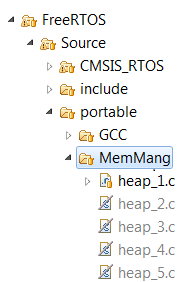
\includegraphics[width=0.2\textwidth]{Pictures/Eclipse/Heaps.png}
	\caption{Einbindung von Heap1. Heap2 bis Heap5 sind vom Build ausgeschlossen}
	\label{fig:HeapsEclipse}
\end{figure}

\begin{lstlisting}[caption={Implementierung von malloc() und free() in Heap1}, linewidth=8cm,captionpos=b, label=lst:heap1, float=hbt]
//**MALLOC**
void *pvPortMalloc( size_t xWantedSize )
{
void *pvReturn = NULL;
static uint8_t *pucAlignedHeap = NULL;
	/* Ensure that blocks are always aligned to the required number of bytes. */
	#if( portBYTE_ALIGNMENT != 1 ){
		if( xWantedSize & portBYTE_ALIGNMENT_MASK )	{
			/* Byte alignment required. */
			xWantedSize += ( portBYTE_ALIGNMENT - ( xWantedSize & portBYTE_ALIGNMENT_MASK ) );
		}
	}
	#endif
	vTaskSuspendAll();
	if( pucAlignedHeap == NULL ){
		/* Ensure the heap starts on a correctly aligned boundary. */
		pucAlignedHeap = ( uint8_t * ) ( ( ( portPOINTER_SIZE_TYPE ) &ucHeap[ portBYTE_ALIGNMENT ] ) & ( ~( ( portPOINTER_SIZE_TYPE ) portBYTE_ALIGNMENT_MASK ) ) );
	}
	/* Check there is enough room left for the allocation. */
	if( ( ( xNextFreeByte + xWantedSize ) < configADJUSTED_HEAP_SIZE ) &&
		( ( xNextFreeByte + xWantedSize ) > xNextFreeByte )	)	{
		/* Return the next free byte then increment the index past this
		block. */
		pvReturn = pucAlignedHeap + xNextFreeByte;
		xNextFreeByte += xWantedSize;
	}
	xTaskResumeAll();
	return pvReturn;
}

//**FREE**
void vPortFree( void *pv )
{
	/* Memory cannot be freed using this scheme. */
	( void ) pv;
	/* Force an assert as it is invalid to call this function. */
	configASSERT( pv == NULL );
}

\end{lstlisting}

   
Diese stellen prinzipiell schon die ge\-läu\-figsten Implementierungen zur Speicherverwaltung. Es bleibt aber auch weiterhin die Möglichkeit seine eigene Speicherverwaltung zu implementieren. In dieser Arbeit werden wir Heap1 etwas genauer betrachten um ein grund\-sätz\-liches Verständnis für die FreeRTOS Speicherverwaltung zu bekommen. Heap2 - Heap 5 werden nur kurz beschrieben und können im Detail in \cite{MasteringFreeRTOS}\cite{FreeRTOSAdvanced} nachgelesen werden.      
Wie schon am Anfang dieses Abschnitts beschrieben, werden für alle RTOS Objekte Speicher benötigt, der Speicher für Objekte wie Semaphore und Tasks wird automatisch in den Erzeugerfunktionen alloziert, in dem intern die Funktion \textit{pvPortMalloc()} aufgerufen wird. Die Erzeugerfunktion xTaskCreate() beispielsweise, erzeugt eine FreeRTOS Task. Listing \ref{lst:xTaskCreate} zeigt wie \verb|xTaskCreate()| die Funktion \verb|pvPortMalloc()| verwendet (Zeile 5, 11) um Speicher für den Stack und den Task Control Block zu allozieren.
\begin{lstlisting}[caption={xTaskCreate() memory allocation. Aus Task.c}, linewidth=8cm,captionpos=b, label=lst:xTaskCreate, float=hbt]
StackType_t *pxStack;
/* Allocate space for the stack 
used by the task being created. */
pxStack = 
( StackType_t * ) pvPortMalloc(( ( ( size_t ) usStackDepth ) 
* sizeof( StackType_t ) ) );

if( pxStack != NULL )
{
	/* Allocate space for the TCB. */
	pxNewTCB = ( TCB_t * ) pvPortMalloc( sizeof( TCB_t ) );

	if( pxNewTCB != NULL )
	{
		/* Store the stack location in the TCB. */
		pxNewTCB->pxStack = pxStack;
	}
//...
}
\end{lstlisting}
Alle Objekte die mittels pvPortMalloc() alloziert werden, darunter auch der Kernel selbst, teilen sich einen gemeinsamen Adressraum, siehe Abbildung \ref{fig:AddressSpace}. Eine Speicherzugriffsverletzung ist somit durchaus möglich. In Abschnitt \ref{sec:Memory Protection} wird gezeigt welche Möglichkeit der STM32F4 und FreeRTOS bieten um Speicherzugriffe sicherer zu gestalten.    
\begin{figure}[htb!]
	\centering
		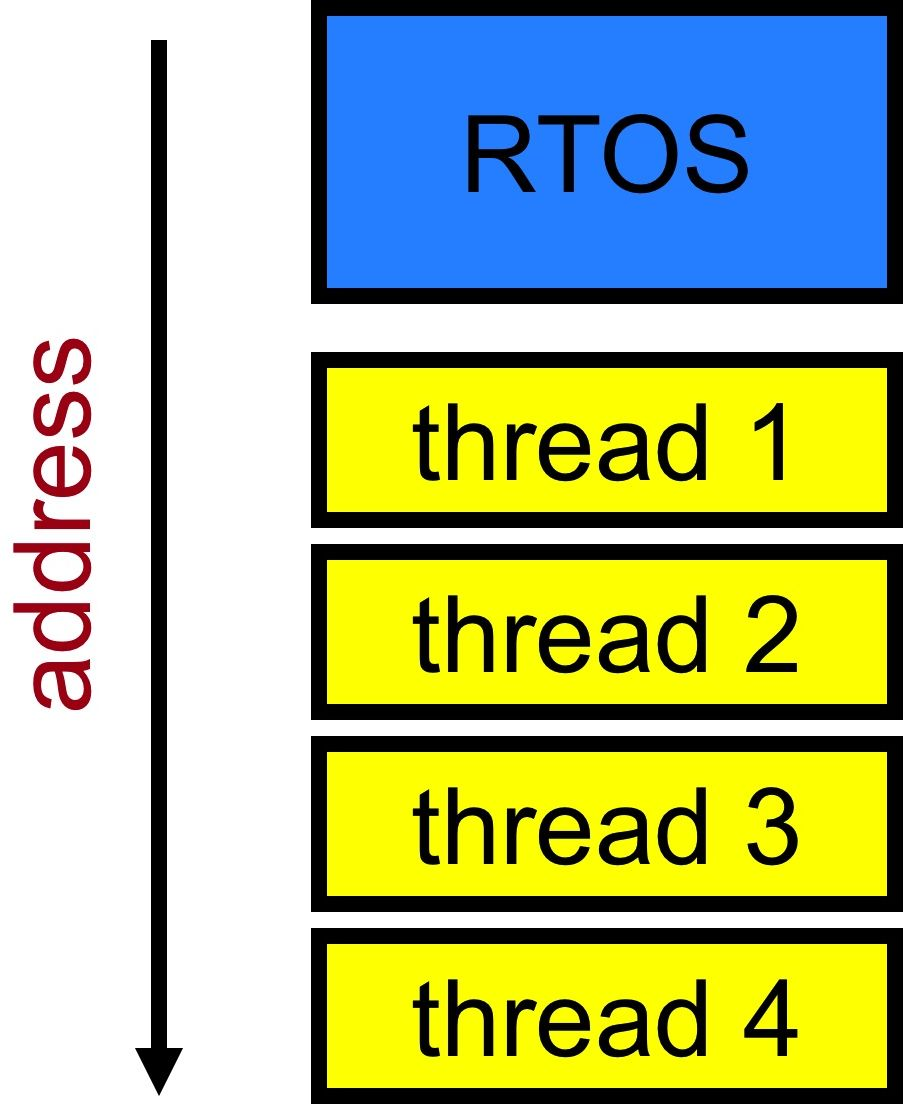
\includegraphics[width=0.2\textwidth]{Pictures/EmbeddedCom/addressSpace.jpg}
	\caption{Adressraum FreeRTOS und Tasks}
	\quelle{Colin Walls - Embedded.com}
	\label{fig:AddressSpace}
\end{figure}    
\subsubsection{FreeRTOS Heap Implementierungen}
Bevor Objekte erzeugt werden können, muss ein Pool an Speicher für die Objekte definiert werden. Die einfachste Form einen Memory Pool zu erzeugen ist ein Array. In FreeRTOS nennt sich dieses Array ucHeap. 
\begin{lstlisting}[label=lst:ucHeap, float=hbt, numbers = none]
static uint8_t ucHeap[ configTOTAL_HEAP_SIZE ];
\end{lstlisting}
\newline
Die Größe des Heaps wird durch das Präprozessor-Define \verb|configTOTAL_HEAP_SIZE | konfiguriert. Die Gesamtgröße berechnet sich wie folgt:
\newline
\newline
MaxHeapSize $=$ configTOTAL\_HEAP\_SIZE $\ast$ Wortbreite\footnote{Beim STM32F4 ist die Wortbreite 32 bit} 
\newline
\newline
Die Speicherverwaltung durch Heap1 ist sehr einfach. Heap1 deklariert lediglich die Funktion pvPortMalloc(). Die Funktion pvPortFree() wird nicht ausimplementiert. Abbildung \ref{fig:Heap1} zeigt wie sich der Speicher nach dem Erzeugen von zwei Tasks aussieht. Für jede Task wird ein TCB und ein Stack erzeugt, die Speicherobjekte liegen direkt hintereinander, da pvPortFree() nicht implementiert ist, kommt es auch nicht zu einer Fragmentierung des Speichers. Diese lineare Speicherzuweisung gilt für alle Objekte die mittels pvPortMalloc() alloziert werden, dazu gehören sowohl RTOS spezifische Objekte als auch Objekte die durch den Benutzer erzeugt werden. 
\begin{figure}[ht!]
	\centering
		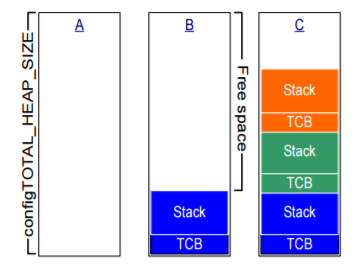
\includegraphics[width=0.3\textwidth]{Pictures/FreeRTOSOrg/heap1Alg.png}
	\caption{Beispiel Speicherbelegung nach drei Instanziierung von Tasks}
	\quelle{FreeRTOS.org}
	\label{fig:Heap1}
\end{figure}
Ein so einfacher Speicheralgorithmus wie Heap1 hat durchaus seine Berechtigung. Bei vielen embedded Anwendungen wird der Speicher für die benötigten Objekte vor dem Start des Schedulers erzeugt. Eine spätere Freigabe von belegten Ressourcen ist nicht nötig, da die Objekte über die gesamte Laufzeit des Programms bestehen sollen. Genau für solche Anwendungen steht Heap1 zur Verfügung. 
Nachfolgend ein Kurzüberblick über die nicht beschriebenen Beispiel Implementierungen.  
\begin{itemize}
	\item Heap2 - Ähnlich Heap1. Erlaubt allerdings Speicherfreigabe durch vPortFree(). Best Fit Algorithmus zur Speicherallozierung. 
	\item Heap3 - Verwendet C Library Malloc() und free() und deaktiviert den Scheduler zur Speicherallozierung.
	\item Heap4 - Ähnlich Heap1 und Heap2. Verwendet First Fit Algorithmus zur Speicherallozierung. Verbindet mehrere kleinere Speicherblöcke zu einem Großen. Minimiert Speicherfragmentierung.
	\item Heap5 - Gleicher Algorithmus wie Heap4 allerdings können mehrere Memory Pools erzeugt werden.
\end{itemize}
\subsubsection{Memory Protection}
\label{sec:Memory Protection}
STM32F4 spezifisch, MPU vorhanden
\begin{figure}[hb!]
	\centering
		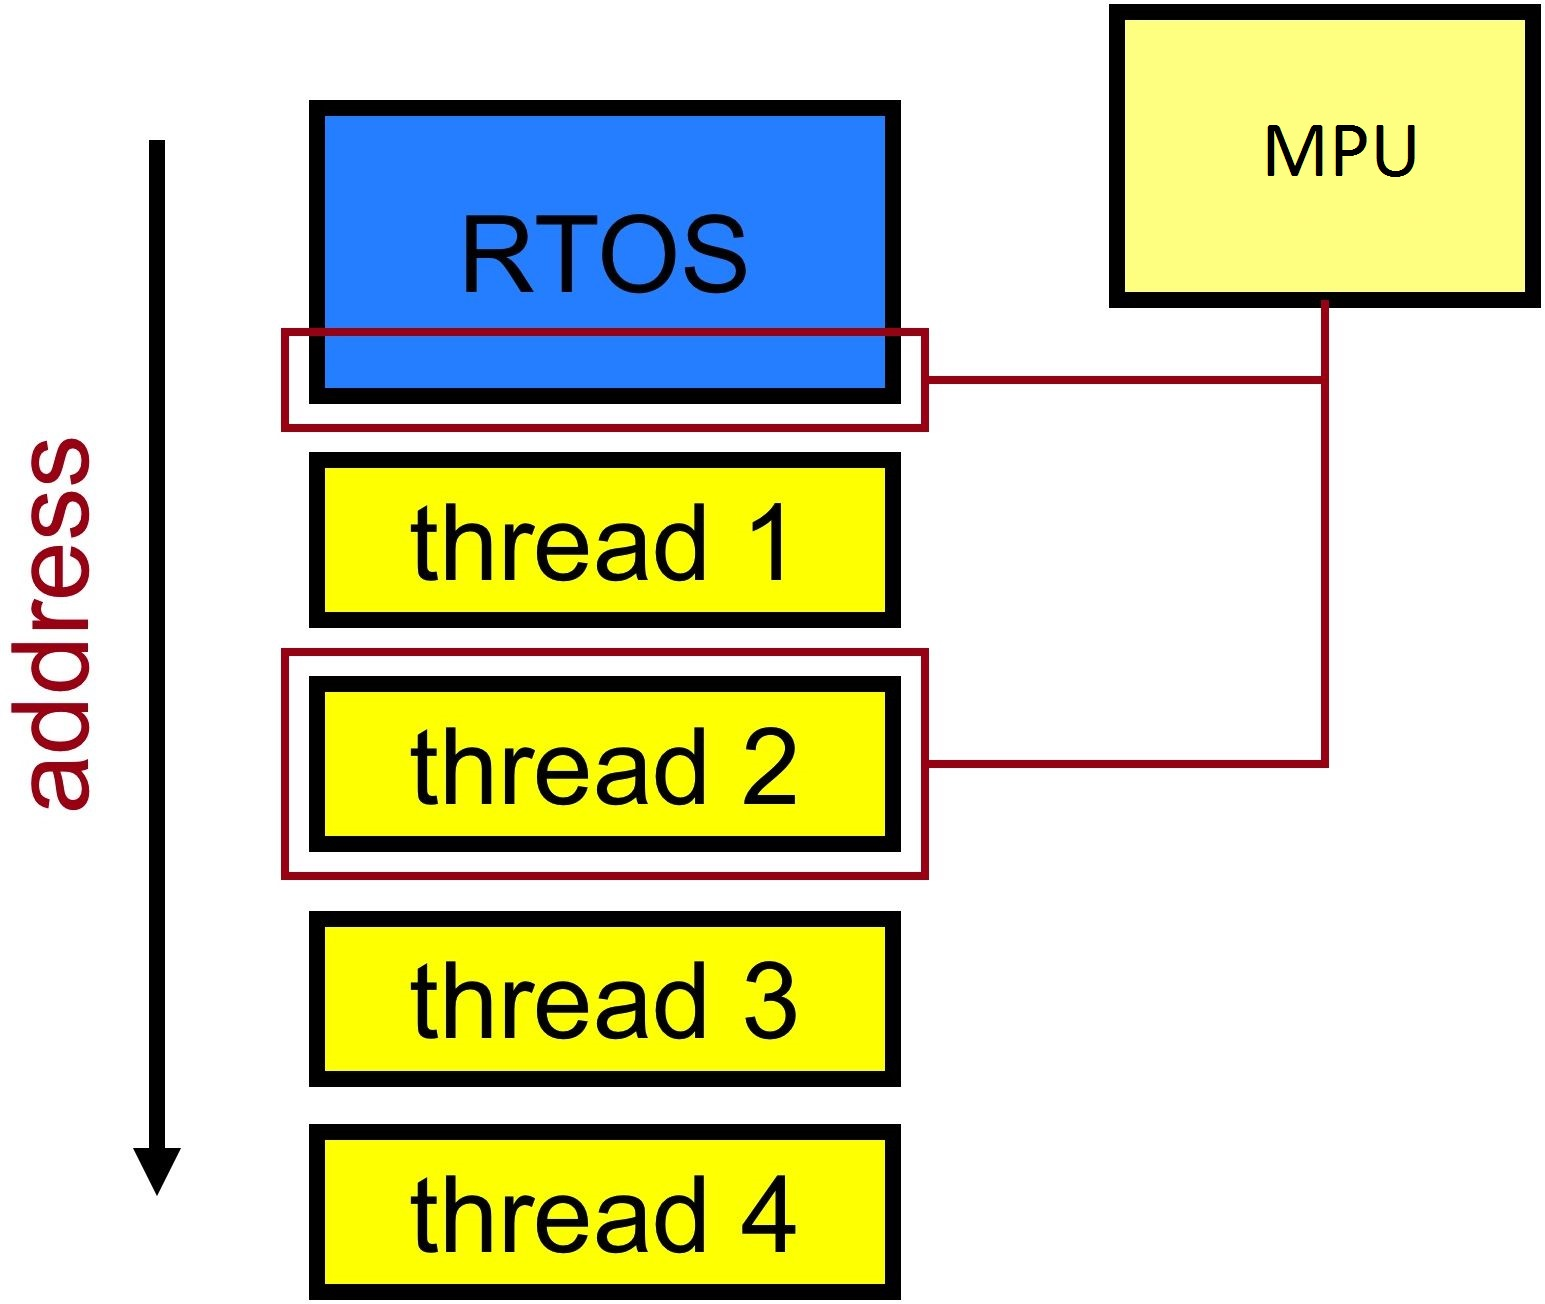
\includegraphics[width=0.3\textwidth]{Pictures/EmbeddedCom/addressSpaceMMU}
	\caption{Adressraum FreeRTOS und Tasks mit Memory Protection}
	\quelle{Colin Walls - Embedded.com}
	\label{fig:AddressSpaceMMU}
\end{figure} 
\subsubsection{Static Memory Allocation}
Die statische Speicherverwaltung wird durch das Präprozessor-Define configSUPPORT\_STATIC\_ALLOCATION 1 in der FreeRTOS\_config aktiviert. Für die statische Objekterzeugung können die dynamischen Erzeugerfunktionen nicht mehr verwendet werden, daher stehen spezielle Erzeugerfuntkionen für die statische Speicherallozierung zur Verfügung, wie xTaskCreateStatic() statt xTaskCreate() oder xSemaphoreCreateBinaryStatic() statt xSemaphoreCreateBinary(). Der Vorteil der statischen Speicherverwaltung ist, dass der Belegte Speicher im RAM schon zur Übersetzungszeit bekannt ist und die potenzielle Fehlerquelle der dynamischen Speicherverwaltung vermieden wird. Nachteil ist, dass mehr RAM verwendet wird als bei den meisten Heap Implementierungen. Heap1 stellt eine geeignete Alternative in der dynamischen Speicherverwaltung.   

      